\documentclass[aspectratio=169,11pt]{beamer}
\usepackage[T1]{fontenc}
\usepackage{lmodern}
\usepackage{amsmath,amssymb}
\usepackage{booktabs}
\graphicspath{{figures/}{../project4/figures/}}  % local copy, or the repo's figures

% ---------------------------------------------------------------- look
\usetheme{default}
\setbeamertemplate{navigation symbols}{}
\definecolor{ink}{HTML}{1F2A37}
\definecolor{accent}{HTML}{2A78D6}
\definecolor{muted}{HTML}{6B7280}
\setbeamercolor{frametitle}{fg=ink}
\setbeamercolor{title}{fg=ink}
\setbeamercolor{structure}{fg=accent}
\setbeamercolor{normal text}{fg=ink}
\setbeamerfont{frametitle}{series=\bfseries,size=\Large}
\setbeamertemplate{itemize items}{\textcolor{accent}{\small$\blacktriangleright$}}
\setlength{\leftmargini}{1.2em}

% Presenter of each slide, shown in the footer. Change one line per slide.
\newcommand{\thepresenter}{}
\newcommand{\presenter}[1]{\renewcommand{\thepresenter}{#1}}
\setbeamertemplate{footline}{%
  \hspace{1em}\textcolor{muted}{\scriptsize\thepresenter}\hfill
  \textcolor{muted}{\scriptsize\insertframenumber/\inserttotalframenumber}\hspace{1em}\vspace{0.6em}}

\newcommand{\cfp}{c_{FP}}
\newcommand{\cfn}{c_{FN}}
\newcommand{\ci}{c_I}
\newcommand{\key}[1]{\textcolor{accent}{\textbf{#1}}}
\DeclareMathOperator{\logit}{logit}

\title{Classification with Unequal Error Costs and Rejection}
\subtitle{MAC F312 Semester Project \textbar{} Group 4}

\begin{document}

% =================================================================== 1
\presenter{Vismay V Shanbhag}
\begin{frame}[plain]
\vspace{1.5em}
{\usebeamerfont{title}\usebeamercolor[fg]{title}\huge\bfseries Classification with Unequal\\[2pt] Error Costs and Rejection\par}
\vspace{0.6em}
{\large\textcolor{muted}{MAC F312 Semester Project \textbar{} Group 4}\par}
\vspace{1.8em}
\small
\begin{tabular}{@{}ll@{\hspace{3em}}ll@{}}
Mohammad Zaid Agha & 2024ADPS0840G & Saatwik Tiwari & 2024ADPS0878G\\
Nitin Sureshkumar & 2024ADPS0881G & Lakshya Satya & 2024ADPS0828G\\
Tanishk Milind Tasgaonkar & 2024ADPS0874G & Vismay V Shanbhag & 2024ADPS0876G\\
\end{tabular}
\vfill
\textcolor{muted}{\footnotesize A spam filter judged by what its mistakes cost, not by how many it makes.}
\end{frame}

% =================================================================== 2
\presenter{Vismay V Shanbhag}
\begin{frame}{The problem: three actions, unequal costs}
\begin{columns}[T]
\begin{column}{0.42\textwidth}
For every email the filter chooses one action:
\begin{itemize}
  \item \key{deliver} it to the inbox
  \item send it to the \key{spam folder}
  \item hold it for a person to \key{inspect}
\end{itemize}
\vspace{0.5em}
A spam in the inbox is a nuisance.\\
A real email in the spam folder may never be seen.
\end{column}
\begin{column}{0.54\textwidth}
\centering
\begin{tabular}{lcc}
\toprule
Action & real ($y=0$) & spam ($y=1$)\\
\midrule
deliver & $0$ & $\cfn=1$\\
spam folder & $\cfp=10$ & $0$\\
inspect & $\ci=0.3$ & $\ci=0.3$\\
\bottomrule
\end{tabular}
\vspace{1em}

\fbox{\parbox{0.9\linewidth}{\centering\small We report the \key{realized loss}:\\
the average cost per held-out email.}}
\end{column}
\end{columns}
\end{frame}

% =================================================================== 3
\presenter{Vismay V Shanbhag}
\begin{frame}{One shared pipeline for every experiment}
\begin{columns}[T]
\begin{column}{0.5\textwidth}
\textbf{Data and splits} (\texttt{data.py})
\begin{itemize}
  \item UCI Spambase: 4{,}601 emails, 39.4\% spam, 57 features
  \item Stratified 60/20/20 splits: 2{,}761 / 921 / 919
  \item 20 seeds; report mean $\pm$ standard error
  \item Fit on train, choose on validation, report on test only
\end{itemize}
\end{column}
\begin{column}{0.48\textwidth}
\textbf{Decisions and scoring}
\begin{itemize}
  \item \texttt{decision.py}: loss matrix $\to$ thresholds $\to$ action
  \item \texttt{metrics.py}: realized loss, accuracy, inspection rate, confusion with an inspect column
  \item Checked against brute force on 10{,}000 random cases
\end{itemize}
\end{column}
\end{columns}
\vspace{0.8em}
\centering
\begin{tabular}{lcc}
\toprule
Loss matrix $L$ & real ($y=0$) & spam ($y=1$)\\
\midrule
deliver & $0$ & $\cfn$\\
spam folder & $\cfp$ & $0$\\
inspect & $\ci$ & $\ci$\\
\bottomrule
\end{tabular}\\[0.6em]
{\small Parameters: $\cfp=10$, \ $\cfn=1$, \ $\ci=0.3$}
\end{frame}

% =================================================================== 4
\presenter{Mohammad Zaid Agha}
\begin{frame}{Choosing the cheapest action}
\small
With spam probability $p$ the expected costs are: deliver $\cfn p$, \ spam $\cfp(1-p)$, \ inspect $\ci$. Pick the lowest line.
\begin{columns}[T]
\begin{column}{0.48\textwidth}
\begin{itemize}
  \item deliver if $p\le \ci/\cfn = \key{0.3}$
  \item spam folder if $p\ge 1-\ci/\cfp = \key{0.97}$
  \item inspect in between
\end{itemize}
\end{column}
\begin{column}{0.48\textwidth}
\begin{itemize}
  \item no inspection: one cut at $t^\ast=\tfrac{\cfp}{\cfp+\cfn}=\tfrac{10}{11}$, not $0.5$
  \item inspection used only if $\ci<c^\ast=\tfrac{\cfp\cfn}{\cfp+\cfn}=\tfrac{10}{11}$
\end{itemize}
\end{column}
\end{columns}
\centering
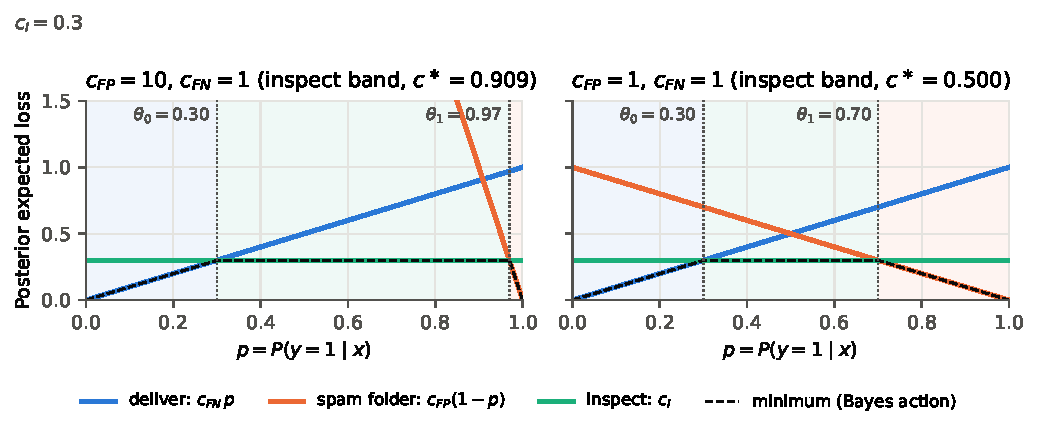
\includegraphics[width=0.68\textwidth]{t1_expected_loss.pdf}\\
{\scriptsize\textcolor{muted}{Left: $\ci=0.3$. Right: $\ci=1$, where inspection never wins.}}
\end{frame}

% =================================================================== 5
\presenter{Nitin Sureshkumar}
\begin{frame}{Model 1: logistic regression}
The rule needs a probability $p$ for every email. The first model gives it directly:
\[ p = \sigma(w^\top x + b) \]
\begin{itemize}
  \item Fitted by \key{Newton's method} (iteratively reweighted least squares), written from scratch
  \item \key{L2 penalty} on $w$ (not the intercept), chosen on validation log-loss from $10^{-2}$ to $10^{3}$
  \item The penalty keeps the weights finite even when the classes are separable
  \item Converges in a few iterations
\end{itemize}
\vspace{0.5em}
\textbf{Tests:} zero gradient at the solution, matches scikit-learn, recovers the true weights from a large simulated sample.
\end{frame}

% =================================================================== 6
\presenter{Tanishk Milind Tasgaonkar}
\begin{frame}{Model 2: Gaussian classifiers}
Model what each class looks like, then use Bayes' rule to get $p$.
\begin{columns}[T]
\begin{column}{0.48\textwidth}
\begin{itemize}
  \item \key{Shared} covariance $\Rightarrow$ linear boundary
  \item \key{Class-specific} covariance $\Rightarrow$ quadratic boundary
\end{itemize}
\end{column}
\begin{column}{0.48\textwidth}
\begin{itemize}
  \item Many Spambase features are almost always 0 $\Rightarrow$ singular covariances
  \item Shrinkage: $S\mapsto(1-\alpha)S+\alpha\frac{\operatorname{tr}S}{d}I$, $\alpha$ chosen on validation
\end{itemize}
\end{column}
\end{columns}
\vspace{0.8em}
\begin{itemize}
  \item All densities in the log domain from Cholesky factors; no matrix is inverted
  \item Agrees with scikit-learn's LDA to $10^{-8}$ and QDA to $10^{-6}$
\end{itemize}
\end{frame}

% =================================================================== 7
\presenter{Tanishk Milind Tasgaonkar}
\begin{frame}{Word counts are not Gaussian: try $\log(1+x)$}
\begin{columns}[c]
\begin{column}{0.44\textwidth}
\footnotesize\setlength{\tabcolsep}{4pt}
\begin{tabular}{llcc}
\toprule
Features & Model & Log-loss & Cost\\
\midrule
raw & shared & 0.305 & 0.172\\
raw & class-spec. & 0.619 & 0.337\\
$\log(1+x)$ & shared & \key{0.223} & \key{0.143}\\
$\log(1+x)$ & class-spec. & 0.354 & 0.279\\
\bottomrule
\end{tabular}\\[2pt]
{\scriptsize\textcolor{muted}{Test means over 20 splits; cost of the rule with inspection, $\ci=0.3$.}}
\vspace{0.6em}
\begin{itemize}
  \item The transform helps both models
  \item Class-specific stays worse: a $57\times57$ covariance per class needs heavy shrinkage ($\alpha\approx0.9$)
  \item Later sections use the \key{shared model with $\log(1+x)$}
\end{itemize}
\end{column}
\begin{column}{0.54\textwidth}
\includegraphics[width=\linewidth]{c2_gaussian_log1p.pdf}
\end{column}
\end{columns}
\end{frame}

% =================================================================== 8
\presenter{Nitin Sureshkumar}
\begin{frame}{Accuracy rule or cost rule?}
\vspace{-0.4em}
\small
Sweep the cost ratio $r=\cfp/\cfn$ from $1/20$ to $20$ ($\ci=0.1$); apply three rules to the same probabilities.
\begin{columns}[T]
\begin{column}{0.48\textwidth}
\begin{itemize}
  \item \key{The accuracy rule is right only at $r=1$.} Logistic on Spambase: $0.166$ vs $0.082$ at $r=0.1$, $0.115$ vs $0.082$ at $r=10$
  \item \key{Inspection is cheapest everywhere}: $0.050$--$0.053$, inspecting 23--32\%
\end{itemize}
\end{column}
\begin{column}{0.48\textwidth}
\begin{itemize}
  \item Logistic regression is the best model on Spambase with every rule
  \item On synthetic data the correct (quadratic) model is within $0.001$ of the oracle
\end{itemize}
\end{column}
\end{columns}
\vspace{0.2em}
\centering
\includegraphics[width=0.97\textwidth]{task2_loss_spambase.png}
\end{frame}

% =================================================================== 9
\presenter{Lakshya Satya}
\begin{frame}{Can the probabilities be trusted?}
\vspace{-0.6em}
\begin{columns}[c]
\begin{column}{0.56\textwidth}
\small
Our rule compares $p$ with $0.3$ and $0.97$, so $p$ must be \key{calibrated}.
\begin{itemize}
  \item Logistic beats Gaussian on Spambase: log-loss $0.185$ vs $0.224$, ECE $0.021$ vs $0.039$, cost $0.124$ vs $0.142$, with accuracies only 1.3 points apart
  \item Platt scaling fixes much of it: Gaussian cost $0.142\to0.132$
\end{itemize}
\textbf{Same accuracy, different cost} (temperature scaling):\\[2pt]
\footnotesize\setlength{\tabcolsep}{4pt}
\begin{tabular}{lccc}
\toprule
Temperature & Accuracy & Log-loss & Cost\\
\midrule
$T=0.4$ (over-confident) & 0.936 & 0.289 & \key{0.164}\\
$T=1$ (as fitted) & 0.936 & 0.185 & 0.124\\
$T=2.5$ (under-confident) & 0.936 & 0.249 & 0.149\\
\bottomrule
\end{tabular}
\end{column}
\begin{column}{0.4\textwidth}
\centering
\includegraphics[width=\linewidth]{c4_reliability.pdf}
\end{column}
\end{columns}
\end{frame}

% =================================================================== 10
\presenter{Lakshya Satya}
\begin{frame}{When the share of spam changes}
\vspace{-0.4em}
Trained where 39\% is spam, deployed where 5\% is: the probabilities overstate spam.\\[4pt]
If spam still looks the same, every email's log-odds moves by the same amount:
\[
p'=\sigma\big(\logit p+\Delta\big),\qquad
\Delta=\log\frac{\pi_1'}{1-\pi_1'}-\log\frac{\pi_1}{1-\pi_1}
\]
\vspace{-0.6em}
\begin{columns}[c]
\begin{column}{0.36\textwidth}
\small
Example: trained at $\pi_1=0.5$, deployed at $\pi_1'=0.1$:
$p=0.98\ \to\ p'\approx0.845$.\\[3pt]
The email is now \key{inspected} instead of filed as spam.\\[3pt]
Equivalently, move the thresholds instead of the probabilities.
\end{column}
\begin{column}{0.62\textwidth}
\includegraphics[width=\linewidth]{t5_prior_correction.pdf}
\end{column}
\end{columns}
\end{frame}

% =================================================================== 11
\presenter{Mohammad Zaid Agha}
\begin{frame}{Testing the correction}
\vspace{-0.6em}
\begin{columns}[c]
\begin{column}{0.42\textwidth}
\small
Resample the test set to a new spam rate $\pi_1'$; decide with uncorrected, corrected (true $\pi_1'$) and corrected (\key{EM-estimated} $\pi_1'$) probabilities.
\begin{itemize}
  \item At $\pi_1'=0.05$ the correction \key{more than halves} the cost: Spambase $0.095\to0.038$ (logistic), $0.108\to0.051$ (Gaussian)
  \item Uncorrected filter inspects 43--49\% of synthetic emails; corrected: 1.6\%
  \item EM works if the model is calibrated: logistic's estimate is off by only $0.007$--$0.013$
\end{itemize}
\end{column}
\begin{column}{0.56\textwidth}
\includegraphics[width=\linewidth]{c5_prior_shift.pdf}
\end{column}
\end{columns}
\end{frame}

% =================================================================== 12
\presenter{Vismay V Shanbhag}
\begin{frame}{An exact model: accuracy versus cost}
\begin{columns}[T]
\begin{column}{0.44\textwidth}
\footnotesize
Real $x\sim N(-1,1)$, spam $x\sim N(+1,1)$, 40\% spam $\Rightarrow p=\sigma(2x+\lambda)$. Thresholds on $p$ become cuts on $x$, so every rate is a normal CDF: \key{no fitting, no noise}.\\[3pt]
\setlength{\tabcolsep}{3.5pt}
\begin{tabular}{lccc}
\toprule
Rule & Accuracy & Cost & Inspected\\
\midrule
$t=0.5$ & \key{0.846} & 0.772 & 0\\
$t^\ast=10/11$ & 0.739 & 0.311 & 0\\
always deliver & 0.600 & 0.400 & 0\\
with inspection & -- & \key{0.179} & 0.416\\
\bottomrule
\end{tabular}
\begin{itemize}
  \item The most accurate rule costs more than delivering everything
  \item Between $0.5$ and $10/11$, raising the cut lowers accuracy \emph{and} cost
  \item Best cost rises with $\ci$; its slope is the inspection rate; inspection stops at $c^\ast=10/11$ for every $\mu$
\end{itemize}
\end{column}
\begin{column}{0.54\textwidth}
\centering
\includegraphics[width=0.9\linewidth]{t6_accuracy_vs_cost.pdf}\\[2pt]
\includegraphics[width=0.9\linewidth]{t6_risk_reject_vs_cinsp.pdf}
\end{column}
\end{columns}
\end{frame}

% =================================================================== 13
\presenter{Saatwik Tiwari}
\begin{frame}{Do fitted models match the exact model?}
\vspace{-0.4em}
Draw 10{,}000 emails from the exact model per split, fit both models, apply all rules.
\begin{columns}[c]
\begin{column}{0.4\textwidth}
\small
\begin{itemize}
  \item Moving the cut from $0.5$ to $10/11$: accuracy $84.6\%\to73.9\%$, cost $0.780\to0.309$
  \item At $\ci=0.3$ the exact model predicts \key{0.179} with 41.6\% inspected; the fitted Gaussian gives \key{0.181} with 41.7\%
  \item The curves agree at every inspection price
\end{itemize}
\end{column}
\begin{column}{0.58\textwidth}
\includegraphics[width=\linewidth]{c6_inspection_synthetic.pdf}
\end{column}
\end{columns}
\end{frame}

% =================================================================== 14
\presenter{Saatwik Tiwari}
\begin{frame}{Inspection pays on real data}
\vspace{-0.6em}
\begin{columns}[c]
\begin{column}{0.44\textwidth}
\small
Spambase, $\ci=0.3$:\\[3pt]
\footnotesize\setlength{\tabcolsep}{4pt}
\begin{tabular}{lccc}
\toprule
Model & No insp. & With insp. & Inspected\\
\midrule
Gaussian & 0.293 & 0.172 & 25.5\%\\
Logistic & 0.261 & \key{0.161} & 24.1\%\\
\bottomrule
\end{tabular}
\vspace{0.5em}
\begin{itemize}
  \item Saving of $0.10$--$0.12$ per email
  \item The saving shrinks as inspection gets dearer and vanishes at $\ci=10/11$
  \item \key{Not an artefact of duplicates}: without the 9.8\% repeated rows, cost still falls $0.264\to0.160$ (logistic)
\end{itemize}
\end{column}
\begin{column}{0.54\textwidth}
\includegraphics[width=\linewidth]{c6_inspection_spambase.pdf}
\end{column}
\end{columns}
\end{frame}

% =================================================================== 15
\presenter{Saatwik Tiwari}
\begin{frame}{What we learned}
\begin{enumerate}
  \item \key{Accuracy is the wrong target when errors cost different amounts.}\\
        With $\cfp=10$ the right cut is $10/11$, not $0.5$; the most accurate rule was the most expensive.
  \item \key{The rule is only as good as the probabilities.}\\
        Same accuracy, different cost; logistic regression was best calibrated and cheapest.
  \item \key{A change in the spam rate is cheap to fix.}\\
        One log-odds shift more than halved the cost, even with the rate estimated by EM.
  \item \key{Inspection is worth paying for when it is cheap.}\\
        Saves $0.10$--$0.12$ per email at $\ci=0.3$; never used once $\ci\ge10/11$.
\end{enumerate}
\vspace{0.4em}
{\small\textcolor{muted}{Limitations: the inspector is assumed always right, the costs are our choice, and each test set has about 920 emails.}}
\end{frame}

\end{document}
